%%%%%%%%%%%%%%%%%%%%%%%%%%%%%%%%%%%%%%%%%
% Wilson Resume/CV
% XeLaTeX Template
% Version 1.0 (22/1/2015)
%
% This template has been downloaded from:
% http://www.LaTeXTemplates.com
%
% Original author:
% Howard Wilson (https://github.com/watsonbox/cv_template_2004) with
% extensive modifications by Vel (vel@latextemplates.com)
%
% License:
% CC BY-NC-SA 3.0 (http://creativecommons.org/licenses/by-nc-sa/3.0/)
%
%%%%%%%%%%%%%%%%%%%%%%%%%%%%%%%%%%%%%%%%%

%----------------------------------------------------------------------------------------
%	PACKAGES AND OTHER DOCUMENT CONFIGURATIONS
%----------------------------------------------------------------------------------------

\documentclass[10pt]{article} % Default font size

%%%%%%%%%%%%%%%%%%%%%%%%%%%%%%%%%%%%%%%%%
% Wilson Resume/CV
% Structure Specification File
% Version 1.0 (22/1/2015)
%
% This file has been downloaded from:
% http://www.LaTeXTemplates.com
%
% License:
% CC BY-NC-SA 3.0 (http://creativecommons.org/licenses/by-nc-sa/3.0/)
%
%%%%%%%%%%%%%%%%%%%%%%%%%%%%%%%%%%%%%%%%%

%----------------------------------------------------------------------------------------
%	PACKAGES AND OTHER DOCUMENT CONFIGURATIONS
%----------------------------------------------------------------------------------------

\usepackage[a4paper, hmargin=25mm, vmargin=30mm, top=20mm]{geometry} % Use A4 paper and set margins

\usepackage{fancyhdr} % Customize the header and footer

\usepackage{lastpage} % Required for calculating the number of pages in the document

\usepackage{hyperref} % Colors for links, text and headings

\setcounter{secnumdepth}{0} % Suppress section numbering

%\usepackage[proportional,scaled=1.064]{erewhon} % Use the Erewhon font
%\usepackage[erewhon,vvarbb,bigdelims]{newtxmath} % Use the Erewhon font
%\usepackage[utf8]{inputenc} % Required for inputting international characters
\usepackage[T1]{fontenc} % Output font encoding for international characters

\usepackage{fontspec} % Required for specification of custom fonts
% \setmainfont[Path = ./fonts/,
% Extension = .otf,
% BoldFont = Erewhon-Bold,
% ItalicFont = Erewhon-Italic,
% BoldItalicFont = Erewhon-BoldItalic,
% SmallCapsFeatures = {Letters = SmallCaps},
% Ligatures = TeX
% ]{Erewhon-Regular}
\setmainfont[
  Ligatures = TeX,
  BoldFont = Gill Sans,
  BoldItalicFont = Gill Sans Italic]{Gill Sans Light}
\setmonofont[Ligatures = TeX]{Fira Code}

\newfontfamily{\sectionf}[Ligatures = TeX]{Didot}

\usepackage{color} % Required for custom colors
\definecolor{slateblue}{rgb}{0.17,0.22,0.64}

\usepackage{sectsty} % Allows customization of titles
\sectionfont{\color{slateblue}\sectionf} % Color section titles

\fancypagestyle{plain}{\fancyhf{}\cfoot{\thepage\ of \pageref{LastPage}}} % Define a custom page style
\pagestyle{plain} % Use the custom page style through the document
\renewcommand{\headrulewidth}{0pt} % Disable the default header rule
\renewcommand{\footrulewidth}{0pt} % Disable the default footer rule

\setlength\parindent{0pt} % Stop paragraph indentation

% Non-indenting itemize
\newenvironment{itemize-noindent}
{\setlength{\leftmargini}{0em}\begin{itemize}}
{\end{itemize}}

% Text width for tabbing environments
\newlength{\smallertextwidth}
\setlength{\smallertextwidth}{\textwidth}
\addtolength{\smallertextwidth}{-2cm}

\newcommand{\sqbullet}{~\vrule height 1ex width .8ex depth -.2ex} % Custom square bullet point definition

%----------------------------------------------------------------------------------------
%	MAIN HEADER COMMAND
%----------------------------------------------------------------------------------------

\newcommand{\headline}[2]{
{\huge{\color{slateblue}{#1} \sectionf{#2}}}\\ % Header section name and color
\rule{\textwidth}{0.35mm}\\ % Rule under the header
}

%----------------------------------------------------------------------------------------
%	ITEM TITLE
%----------------------------------------------------------------------------------------

\newcommand{\itemtitle}[1]{{\color{slateblue}\sectionf #1}}

%----------------------------------------------------------------------------------------
%	JOB COMMAND
%----------------------------------------------------------------------------------------

\newcommand{\job}[6]{
\begin{tabbing}
\hspace{2cm} \= \kill
\textbf{#1} \> \itemtitle{#5}\\
\textbf{#2} \>\+ \footnotesize{\href{#4}{#3}}\\
\begin{minipage}{\smallertextwidth}
\vspace{2mm}
#6
\end{minipage}
\end{tabbing}
\vspace{2mm}
}

%----------------------------------------------------------------------------------------
%	SKILL GROUP COMMAND
%----------------------------------------------------------------------------------------

\newcommand{\skillgroup}[2]{
\begin{tabbing}
\hspace{5mm} \= \kill
\sqbullet \>\+ \itemtitle{\large #1} \\
\begin{minipage}{\smallertextwidth}
\vspace{2mm}
#2
\end{minipage}
\end{tabbing}
}

%----------------------------------------------------------------------------------------
%	INTERESTS GROUP COMMAND
%-----------------------------------------------------------------------------------------

\newcommand{\interestsgroup}[1]{
\begin{tabbing}
\hspace{5mm} \= \kill
#1
\end{tabbing}
\vspace{-10mm}
}

\newcommand{\interest}[1]{\sqbullet \> \textbf{#1}\\[3pt]} % Define a custom command for individual interests

%----------------------------------------------------------------------------------------
%	TABBED BLOCK COMMAND
%----------------------------------------------------------------------------------------

\newcommand{\tabbedblock}[1]{
\begin{tabbing}
\hspace{2cm} \= \hspace{4cm} \= \kill
#1
\end{tabbing}
} % Include the file specifying document layout
\newcommand{\maincolwidth}{13cm}
\usepackage{tikz}

%----------------------------------------------------------------------------------------

\begin{document}

%----------------------------------------------------------------------------------------
%	NAME AND CONTACT INFORMATION
%----------------------------------------------------------------------------------------

\headline{Stephan}{Brandauer} % Print the main header

%------------------------------------------------

\vspace{-2mm}\hfill\emph{\sectionf{Computer Science and Software Development.}}\\[7mm]
\newcommand{\maillink}[1]{\href{mailto:#1}{\texttt{#1}}}

\begin{center}
  \begin{tabular}{rl|rl}
    \itemtitle{Address}     & Dag Hammarkj\"o{}lds v. 29A, & \itemtitle{Phone}  & +46 700 599 236 \\
                            & 752 37 Uppsala,   & \hspace{4mm}\itemtitle{E-Mail} & \maillink{stephan.brandauer@gmail.com} \\
                            & Sweden            & \itemtitle{Web}     & \url{http://stbr.me} \\
    \itemtitle{Nationality} & Austrian      & \itemtitle{Other}  & \href{https://twitter.com/sbrandauer}{
\includegraphics[height=1em,trim={30mm 34mm 0 13mm},clip]{twitter.eps}\texttt{sbrandauer}}, \href{https://github.com/kaeluka}{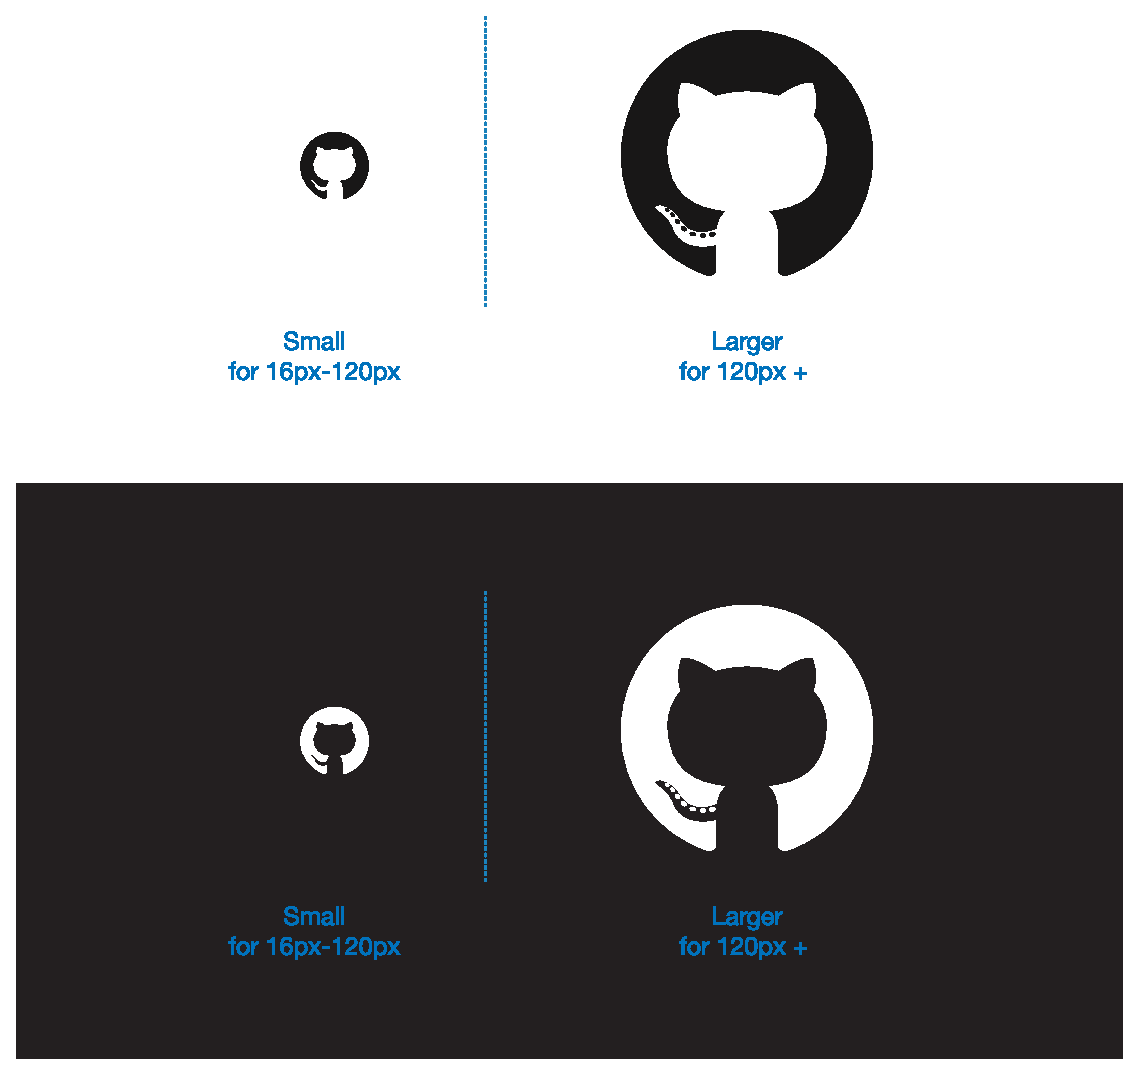
\includegraphics[height=1em,trim={48mm 145mm 127mm 16mm},clip]{github.eps} \texttt{kaeluka}} \\
    \itemtitle{Languages}   & German (\emph{native}), English (\emph{fluent}) & & \href{https://www.linkedin.com/in/stephan-brandauer}{
\includegraphics[height=0.8em]{linkedin.eps} \texttt{stephan-brandauer}} \\
                            & Swedish (\emph{basic working proficiency})\hspace{4mm}
  \end{tabular}
\end{center}
% ----------------------------------------------------------------------------------------
%	PERSONAL PROFILE
%----------------------------------------------------------------------------------------

\section{Personal Profile}

{I have recently defended (opponent: Prof. Doug Lea, SUNY) my PhD in computer
  science at Uppsala University, Sweden. My research has focused on aliasing
  (several variables holding references to the same datum) in imperative
  programming languages. Aliasing makes both writing, understanding, and
  optimising code hard. Aliasing has been the common theme that has been tying
  together my research spanning from \textbf{type system/language design} to
  \textbf{dynamic analysis of program corpora} to a domain-specific language for
  \textbf{data structure-design and -optimisation}.

  I deeply care about program performance, but I also think that most
  programmers shouldn't need to. To this end, I've been trying to find ways to
  constrain high level languages in just the right way: constraints that don't
  hurt writing code in practise, yet give enough information to compiler,
  runtime, or framework to do optimisations that can provide great program
  performance.

  Although my research work's focus has been quite narrow, at this point I'm
  mainly interested in getting experience in software engineering: I want to
  learn all about how your team works together, the business domains you're
  solving, how you're communicating with your customers. Basically: all the good
  things I have missed out on during my PhD. }

%----------------------------------------------------------------------------------------
%	EDUCATION SECTION
%----------------------------------------------------------------------------------------

\newcommand{\project}[1]{\emph{#1}}
\newcommand{\ddomains}{\project{Disjointness Domains}}
\newcommand{\spencer}{\project{Spencer}}
\newcommand{\cflat}{\project{$C\flat$}}
\newcommand{\encore}{\project{Encore}}

\section{Education}

\tabbedblock{ \bf{2013-2018} \> PhD in Computer Science (defended in Jan, 2019)
  -
  \href{http://katalog.uu.se/empinfo/?id=N12-145}{Uppsala University} \\[5pt]
  \> Research on programming language design, analysis, and implementation. \\
  \> \hspace*{-5mm}\parbox{12cm}{
    \begin{itemize}
      \renewcommand{\labelitemi}{\sqbullet}
    \item I designed \ddomains{}, a type system to express fine grained
      alias invariants in data structures.
    \item I designed and implemented \spencer{}, a dynamic analysis tool that runs real
      world Java software, collects extensive program traces and lets users analyse
      these traces using a specifically designed \emph{domain-specific language}
      executed by a \emph{web service}.
    \item I designed and implemented \cflat{}, a domain-specific
      language and compiler using Java's annotation framework that let users
      implement data structures that are simple, have good performance, and can
      adapt their performance to match a wide range of use cases.
    \item I worked, with others, on the compiler of the \encore{} research language, an object
      oriented programming language with concurrently executing actors as objects.
    \end{itemize}}
}

%------------------------------------------------

\tabbedblock{
  \bf{2011-2013}
  \> Master of Science, Computer Science. Uppsala University.\\[5pt]
  \> Degree project: design, implement, and benchmark a mailbox data structure
  for an actor-\\
  \> based language (called ``Joelle'') that permits \emph{parallel
    processing of messages within an actor.}
}

\tabbedblock{
  \bf{2007-2011}
  \> Bachelor of Science, Cognitive Informatics. Bielefeld University.\\[5pt]
  \> Degree project: Build a 2D rigid body and particle physics engine with an interactive UI.
}

%----------------------------------------------------------------------------------------
%	EMPLOYMENT HISTORY SECTION
%----------------------------------------------------------------------------------------

\section{Selected Publications}
%\newcommand{\paperentry}[6]{\bf{#1}\>\itemtitle{#2}\\\>\parbox{\maincolwidth}{\footnotesize{\emph{#3}}}\\\>\parbox{10cm}{\footnotesize{#4}}\\[1mm]\>\parbox{10cm}{#5}\\[1mm]\>\footnotesize{\url{#6}}\\[5mm]}
\newcommand{\barepaperentry}[5]{\bf{#1}\>\parbox{\maincolwidth}{\itemtitle{#2}}\\\>\parbox{\maincolwidth}{\footnotesize{\emph{#3}}}\\[1mm]\>\parbox{\maincolwidth}{\footnotesize{#4}}\\[1mm]\>\parbox{\maincolwidth}{#5}}
\newcommand{\paperentry}[6]{\barepaperentry{#1}{#2}{#3}{#4}{#5}\\[1mm]\>\parbox{\maincolwidth}{\footnotesize{\url{#6}}}\\[5mm]}
\newcommand{\linklesspaperentry}[6]{\barepaperentry{#1}{#2}{#3}{#4}{#5}\\[5mm]}

\newcommand{\papersgroup}[1]{\begin{tabbing}\hspace{2cm} \= \hspace{8cm} \=\kill#1\end{tabbing}}

\papersgroup{
  \paperentry
  {Onward!'18}
  {\cflat{}: A New Approach to Efficient and Tunable Collections}
  {St. Brandauer, E. Castegren, T. Wrigstad}
  {Onward!: Symposium on New Ideas in Programming and Reflections on Software
    2018. Boston, USA.}
  {A domain specific language to develop data structures that are simple, have
    good performance, and can adapt to many different use cases.}
  {http://stbr.me/cflat}

  \paperentry
  {MSR'17}
  {Spencer: Interactive Heap Analysis for the Masses}
  {St. Brandauer and T. Wrigstad}
  {Int'l Conf. on Mining Software Repositories (MSR) 2017. Buenos Aires, AR.}
  {The paper that introduces the Spencer project.}
  {http://stbr.me/spencer}

  \paperentry
  {QAPL'17}
  {Mining for Safety using Interactive Trace Analysis}
  {St. Brandauer and T. Wrigstad}
  {Workshop on Quantitative Aspects of Programming Languages and Systems (QAPL)
    2017. Uppsala, SE.}
  {An application of Spencer to a corpus of programs, looking
    for safety properties of objects (like uniqueness, immutability, etc).}
  {http://stbr.me/spencer}

  \paperentry
  {SFM'15}
  {Parallel Objects for Multicores: A Glimpse at the Parallel Language Encore}
  {St. Brandauer, E. Castegren, D. Clarke, F. Fernández, E.
    Broch Johnsen, Ka I Pun, S. Lizeth Tapia Tarifa, T. Wrigstad, and A. Yang}
  {15th Int'l School on Formal Methods f. Design of Comp., Comm. and
    Software Systems (SFM) 2015. Bertinoro, IT.}
  {An overview of the Encore language.}
  {http://stbr.me/Encore-Glimpse}

  \paperentry
  {OOPSLA'15}
  {Disjointness Domains for Fine-Grained Aliasing}
  {St. Brandauer, D. Clarke, and T. Wrigstad}
  {Object-Oriented Programming, Systems, Languages and Applications (OOPSLA)
    2015. Pittsburgh, PA, USA.}
  {A novel type system for alias control.}
  {http://stbr.me/Disjointness-Domains-for-Fine-Grained-Aliasing}}

\section{Employment History}

\job
{2013 -}{2018}
{Uppsala University}
{http://katalog.uu.se/empinfo/?id=N12-145}
{PhD Student in programming language design, implementation, analysis.}
{See in Education section above.}

%------------------------------------------------

\job
{Feb 2009 -}{Jun 2010}
{Bielefeld University, AI Group}
{https://www.techfak.uni-bielefeld.de/ags/wbski/hiwis/sbrandau/}
{Research Assistant}
{Work on, and maintain, virtual reality applications for cognitive science
  studies. Teaching assistant (run lab sessions, grade home work assignments).}

%------------------------------------------------

\job
{Sep 2007}{Mar 2008}
{Comet Consulting, Salzburg (now part of Rhomberg)}
{https://www.rhomberg.com/en}
{Freelance Programmer, C\#}
{Develop 3D image recognition algorithms and software in \textbf{C\#} for 3D
  LIDAR scanners to monitor safety procedures at railway tunnel construction
  sites. Much of the job was on-site, but overlap with the social work job was
  during nights and evenings.}

%------------------------------------------------

\job
{Sep 2006}{Mar 2008}
{Laube Sozialpsychiatrische Aktivitäten GmbH}
{http://www.laube.at/}
{Social Work}
{Austrian civil service, as an alternative to being drafted for the military.
  Work with chronically mentally ill people. Learned lots.}

%----------------------------------------------------------------------------------------
%	IT/COMPUTING SKILLS SECTION
%----------------------------------------------------------------------------------------

\section{Software Engineering Skills}

\skillgroup{Programming Languages}{
  \textit{(roughly in order of familiarity)}\\[1mm]
  \textbf{Java} - My go-to language.\\[1mm]
  \textbf{Scala} - have used it on several occasions, for example the \spencer{}
  and \cflat{} DSL-compilers.\\[1mm]
  \textbf{Haskell} - used (and loved) it lots for the first 3 years of my
  PhD studies, working on the \encore{} compiler.\\[1mm]
  \textbf{Rust} - Have implemented a throw-away prototype version of \cflat{}.\\[1mm]
  \textbf{C} - have been teaching basic C to university students every year of my PhD.\\[1mm]
  \textbf{C++} - know the core principles that distinguish it from C (smart
  pointers, RAII, objects, zero-cost abstractions, templates, $\ldots$), but would like to know more.\\[1mm]
  \textbf{SQL (Postgres-SQL)} - have used \textbf{Postgres-SQL} to implement
  complex graph queries in \spencer{}.
}

%------------------------------------------------

\skillgroup{Miscellaneous} {

  \textit{Data Analysis:} I have used \textbf{python/pandas},
  \textbf{Apache Spark} (single node; also \textbf{GraphX}), and \textbf{Postgres}.\\[1mm]
  \textit{Optimisation of JVM code:} optimisation is a big part of my research work on
  \cflat{}. I have used the \textbf{JMH} framework, \textbf{VisualVM}, and \textbf{JITWatch}.\\[1mm]
  \textit{Version control:} mostly using \textbf{git}. Also, although rusty,
  \textbf{Mercurial} and \textbf{SVN}.\\[1mm]
  \textit{Compilers:} I have worked on several \textbf{compilers}: one for a
  general purpose language (\encore{}) and have developed two compilers for
  domain-specific languages (for \spencer{}, compiling to SQL; and for \cflat{},
  compiling to
  Java bytecode).\\[1mm]
  \textit{Java Bytecode:} I have used both the \textbf{\href{foo}{ASM
      framework}} and \textbf{\href{https://bytebuddy.net}{bytebuddy}} to a)
  \textbf{programmatically modify Java programs as they are running}, and b)
  \textbf{generate Java code} from high level specifications.}

\section{Teaching Assistant}
\tabbedblock{
  \bf{Fall '17} \> \sqbullet\hspace{2mm}Imperative and Object Oriented Programming Methodology\\
                \> \sqbullet\hspace{2mm}Secure Computer Systems\\
                \> \sqbullet\hspace{2mm}Introduction to Parallel Programming\\[2mm]
  \bf{Fall '16} \> \sqbullet\hspace{2mm}Imperative and Object Oriented Programming Methodology\\
                \> \sqbullet\hspace{2mm}Algorithms and Data Structures 2\\[2mm]
  \bf{Fall '15} \> \sqbullet\hspace{2mm}Imperative and Object Oriented Programming Methodology\\
                \> \sqbullet\hspace{2mm}Project CS (group project using Scrum and Erlang)\\[2mm]
  \bf{Fall '14} \> \sqbullet\hspace{2mm}Imperative and Object Oriented Programming Methodology\\
                \> \sqbullet\hspace{2mm}Project CS (group project using Scrum and Erlang)\\[2mm]
  \bf{Fall '13} \> \sqbullet\hspace{2mm}Imperative and Object Oriented Programming Methodology\\
}

\section{Community Contributions}
\begin{tabbing}
  \hspace{4cm}\=\kill
  \bf{2017---present}           \> \parbox{7cm}{Co-founder/organiser of ``Papers\&Pizza'', a
                                   semi-regular series of presentations by/for
                                   local PhD students and friends from different groups at
                                   the IT Department at Uppsala University.}\\[2mm]
  \bf{ECOOP'17}                 \> Member of Artifact Evaluation Committee\\[2mm]
  \bf{OOPSLA'16}                \> Member of Artifact Evaluation Committee\\[2mm]
  \bf{Annual Scala Workshop'14} \> Local arrangements\\[2mm]
  \bf{ECOOP'14}                 \> Web master\\[2mm]
  \bf{ECOOP'14}                 \> Student Volunteer Programme: local organiser\\[2mm]
  \bf{various}                  \> Student volunteer
\end{tabbing}


\section{References}
\begin{tabbing}
  \hspace{4cm}\=\hspace{4cm}\=\kill
  \itemtitle{Tobias Wrigstad} \> PhD advisor \> Associate Professor at Uppsala University\\[1mm]
  \maillink{tobias.wrigstad@it.uu.se}\\[1mm]
  He has supervised both my master's and my PhD thesis work.\\[5mm]
  \itemtitle{Sophia Drossopoulou} \> Research collaborator \> Professor at Imperial College London\\[1mm]
  \maillink{s.drossopoulou@imperial.ac.uk}\\[1mm]
  We were both members of the Encore team that involved groups from several
  universities.
\end{tabbing}

\section{Hobbies}
Food (producing and consuming), and photography
(\url{https://www.instagram.com/kaelukaphotos/}).
\end{document}